\section{Results \& Discussion}
only triangle plots

\subsection{Actions from different globular clusters\color{red} better name? \color{black}}
After investigating the orbits at given actions and the time evolution of the integrals of motion we consider all actions and other integrals of motion at our given snapshots. We have a look at the energies and angular momenta of the stars and compare them with the radial actions. Our main goal is to find any systematic signatures for the simulations with \acp{IMBH} that can be considered as the direct evidence of the dynamical effect of the \ac{IMBH} itself. For this reason we investigate selected stars which show an abnormal behaviour in above-mentioned plots and compare them to the rest of data to see where we find them.

\begin{figure}[htbp]
\centering
	\begin{subfigure}{0.475\textwidth}
		\includegraphics[width=\textwidth]{Plots/E_J_r_hist_IMBH1.pdf}
		\caption{SIM 1}
		\label{fig:E_J_r_hist_IMBH1}
	\end{subfigure}
	\hfill
	\begin{subfigure}{0.475\textwidth}
		\includegraphics[width=\textwidth]{Plots/E_J_r_hist_IMBH2.pdf}
		\caption{SIM 2}
		\label{fig:E_J_r_hist_IMBH2}
	\end{subfigure}
	\vskip\baselineskip
	\begin{subfigure}{0.475\textwidth}
		\includegraphics[width=\textwidth]{Plots/E_J_r_hist_noIMBH1.pdf}
		\caption{SIM 3}
		\label{fig:E_J_r_hist_noIMBH1}
	\end{subfigure}
	\hfill
	\begin{subfigure}{0.475\textwidth}
		\includegraphics[width=\textwidth]{Plots/E_J_r_hist_noIMBH2.pdf}
		\caption{SIM 4}
		\label{fig:E_J_r_hist_noIMBH2}
	\end{subfigure}
	\caption{Radial action over energy. In \ref{fig:E_J_r_hist_IMBH1} and \ref{fig:E_J_r_hist_IMBH2} it is plotted for both simulations with \ac{IMBH} and the lower ones are for the simulation without \ac{IMBH}. We find the shape from \ref{fig:E_J_r_hist_noIMBH1} and \ref{fig:E_J_r_hist_noIMBH2} clearly in \ref{fig:E_J_r_hist_IMBH1} and \ref{fig:E_J_r_hist_IMBH2}. But in SIM 1 and SIM 2 there are some stars differing from this shape. Some have high radial actions with nearly no energy while others have high energy with no radial actions.}
	\label{fig:E_J_r_hist}
\end{figure}	
In \ref{fig:E_J_r_hist} we plot the radial action over the energy of the star as histograms for all \acp{GC}. We see clearly some stars outside of the shape. They have either no energy and high radial action (above 500 pc km/s) or no radial action and high energy(below \(-4 \cdot10^{-24}\) \(pc^2/s^2\)). The second ones are stars on circular orbits. 


\begin{figure}[htbp]
\centering
	\begin{subfigure}{0.475\textwidth}
		\includegraphics[width=\textwidth]{Plots/E_J_r_hist_bins_IMBH1.pdf}
		\caption{SIM 1}
		\label{fig:E_J_r_hist_bins_IMBH1}
	\end{subfigure}
	\hfill
	\begin{subfigure}{0.475\textwidth}
		\includegraphics[width=\textwidth]{Plots/E_J_r_hist_bins_IMBH2.pdf}
		\caption{SIM 2}
		\label{fig:E_J_r_hist_bins_IMBH2}
	\end{subfigure}
	\vskip\baselineskip
	\begin{subfigure}{0.475\textwidth}
		\includegraphics[width=\textwidth]{Plots/E_J_r_hist_bins_noIMBH1.pdf}
		\caption{SIM 3}
		\label{fig:E_J_r_hist_bins_noIMBH1}
	\end{subfigure}
	\hfill
	\begin{subfigure}{0.475\textwidth}
		\includegraphics[width=\textwidth]{Plots/E_J_r_hist_bins_noIMBH2.pdf}
		\caption{SIM 4}
		\label{fig:E_J_r_hist_bins_noIMBH2}
	\end{subfigure}
	\caption{Radial action over energy only of binary systems. We see the same distribution of stars as in \ref{fig:E_J_r_hist}.}
	\label{fig:E_J_r_bins_hist}
\end{figure}

\par We might get these high energies from former binaries which were divided earlier. One of the stars could have been captured on a circular orbit near the centre while the other could have been left on an unbound orbit and have left the system. To check this we will plot the same values only for our actual binary systems. As we see in \ref{fig:E_J_r_bins_hist} the binary systems are behaving like single stars. There is no signature that the divergent stars are leftovers of former binaries. 


\begin{figure}[htbp]
\centering
	\begin{subfigure}{0.475\textwidth}
		\includegraphics[width=\textwidth]{Plots/L_J_r_hist_IMBH1.pdf}
		\caption{SIM 1}
		\label{fig:L_J_r_hist_IMBH1}
	\end{subfigure}
	\hfill
	\begin{subfigure}{0.475\textwidth}
		\includegraphics[width=\textwidth]{Plots/L_J_r_hist_IMBH2.pdf}
		\caption{SIM 2}
		\label{fig:L_J_r_hist_IMBH2}
	\end{subfigure}
	\vskip\baselineskip
	\begin{subfigure}{0.475\textwidth}
		\includegraphics[width=\textwidth]{Plots/L_J_r_hist_noIMBH1.pdf}
		\caption{SIM 3}
		\label{fig:L_J_r_hist_noIMBH1}
	\end{subfigure}
	\hfill
	\begin{subfigure}{0.475\textwidth}
		\includegraphics[width=\textwidth]{Plots/L_J_r_hist_noIMBH2.pdf}
		\caption{SIM 4}
		\label{fig:L_J_r_hist_noIMBH2}
	\end{subfigure}
	\caption{Radial action over angular momentum. \ref{fig:L_J_r_hist_noIMBH1} and \ref{fig:L_J_r_hist_noIMBH2} look again very similar to each other with no recognizable substructure. In \ref{fig:L_J_r_hist_IMBH1} and \ref{fig:L_J_r_hist_IMBH2} there are stars above the main shape. In the shape we can clearly see a substructure from about 0.3 to about 0.5 pc\(^2\)/s in nearly the whole radial action range. \color{red} DO YOU HAVE ANY IDEA WHAT STARS COULD BE THERE??? \color{black}}
	\label{fig:L_J_r_hist}
\end{figure}
\par Next we plot the radial actions over the absolute angular momenta of the stars of the simulations again as histograms. In \ref{fig:L_J_r_hist} we can see a shape which seems characteristic. Inside this shape we see some substructure in the \acp{GC} with \ac{IMBH}. The stars outside the shape are the stars which we see in \ref{fig:E_J_r_hist} and \ref{fig:E_J_r_bins_hist} as the stars with no energy and high radial actions. Obviously they don't seem to have a specific angular momentum. 

\par We extract these divergent stars and determine their properties. First we check the positions of their actions depending on their guiding star radii.
\begin{figure}
\centering
	\begin{subfigure}{0.475\textwidth}
		\centering
		\includegraphics[width=\textwidth]{Plots/r_g_J_r_IMBH1.pdf}
		\caption{SIM 1}
		\label{fig:r_g_J_r_IMBH1}
	\end{subfigure}
	\hfill
	\begin{subfigure}{0.475\textwidth}
		\centering
		\includegraphics[width=\textwidth]{Plots/r_g_J_r_IMBH2.pdf}
		\caption{SIM 2}
		\label{fig:r_g_J_r_IMBH2}
	\end{subfigure}
	\vskip\baselineskip
	\begin{subfigure}{0.475\textwidth}
		\centering
		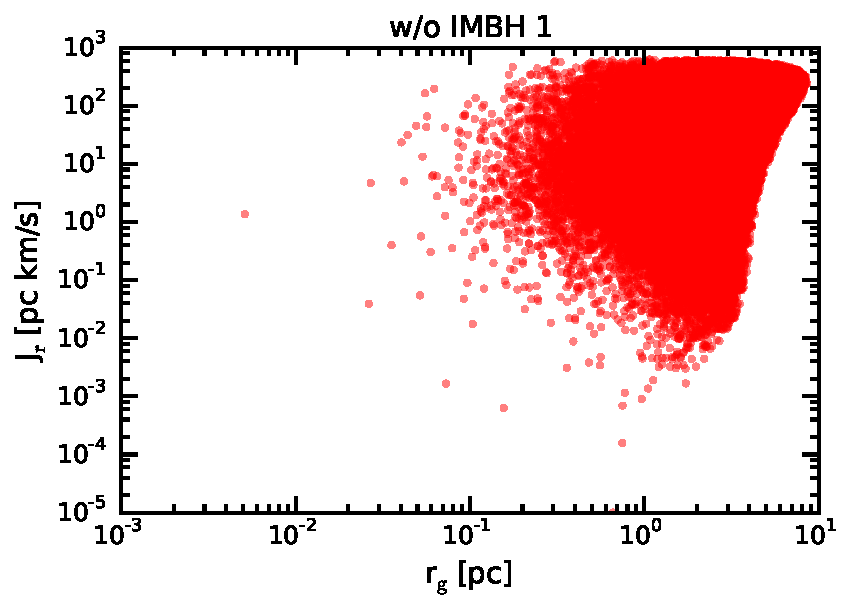
\includegraphics[width=\textwidth]{Plots/r_g_J_r_noIMBH1.pdf}
		\caption{SIM 3}
		\label{fig:r_g_J_r_noIMBH1}
	\end{subfigure}
	\hfill
	\begin{subfigure}{0.475\textwidth}
		\centering
		\includegraphics[width=\textwidth]{Plots/r_g_J_r_noIMBH2.pdf}
		\caption{SIM 4}
		\label{fig:r_g_J_r_noIMBH2}
	\end{subfigure}
	\caption{Radial action over guiding star radius with marked specific stars on loglog scale. All simulations have a similar shaped distributions except for the marked stars which are the specific ones. On the top right corner the shape of \ref{fig:E_J_r_hist_IMBH1} and \ref{fig:E_J_r_hist_IMBH2} is not gently rounded but there are single stars around it. On the lower left there are some extra stars which we identify as the stars with low radial action.}
\end{figure}


\subsection{Discussion \& future perspectives}
do the same distinguishing the mass of the stars\\
redo the work with only observational-like data